% vim: set spell spelllang=es syntax=tex :

\section{Descripción del sistema}

Para aumentar el throughput del sistema se pueden aplicar cuatro enfoques distintos:

\begin{itemize}

	\item 	Dado que en un vídeo ya decodificado el procesamiento de cada
		cuadro es independiente del procesamiento de los demás, y dada
		la disponibilidad de recursos de computo, se pueden procesar
		múltiples cuadros al mismo tiempo sin que esto genere
		diferencias en la información obtenida (salvo por el orden).
		Esto permitiría aumentar la cantidad de cuadros por segundo
		obtenidos, aunque el tiempo de procesamiento de cada uno se
		mantenga igual.

	\item	Para realizar la búsqueda de los objetos, el cuadro puede ser
		dividido. Esto permitirá realizar la búsqueda en cada zona en
		paralelo. Para el correcto funcionamiento, las zonas deberán
		tener partes en común que dependerán del tamaño de los objetos,
		ya que no debe suceder que un objeto no aparezca completo en
		ninguna de las zonas. Esto permitiría reducir el tiempo de
		procesamiento de cada cuadro, ademas de que se puede sacar
		provecho de una mayor localidad espacial.

	\item	Ya que la búsqueda de cada tipo de objetos es independiente de
		la búsqueda de los demás tipos, se pueden realizar múltiples
		búsquedas en paralelo sobre el mismo cuadro por cada tipo de
		objeto.

	\item	Se puede resolver el problema optimizando cada uno de los
		plugins del framework, esperando de esta manera que el tiempo de
		procesamiento de cada cuadro se reduzca lo suficiente como para
		que el sistema pueda procesar la mayoría de los cuadros a
		tiempo.

\end{itemize}

Lamentablemente este último enfoque dificulta su uso como herramienta didáctica,
ya que cada plugin que se agregue o modifique deberá ser optimizado. El primer y
segundo enfoque permiten agregar y modificar los plugins sin mayores
dificultades, y en el caso en el cual un plugin no cumpla con las condiciones
que permitan aplicar alguno de los enfoques, se puede limitar el paralelismo ya
sea no dividiendo el cuadro o procesando solo uno por vez.

Si bien el tercer enfoque es también permitiría agregar o modificar los plugins
fácilmente, en las pruebas que se realizaron se comprobó que realizar las
búsquedas por cada tipo de objeto en paralelo sobre cada fragmento tenia un
efecto adverso. Por este motivo, el tercer enfoque no fue aplicado sobre el
producto final, y no sera incluido en las explicaciones siguientes. Los detalles
de los resultados que llevaron a tomar esta decisión serán detallados mas
adelante en la sección de resultados.

El sistema ejecuta tareas estáticas y tareas dinámicas. Las tareas estáticas son
aquellas que permanecen en ejecución desde el inicio del programa hasta su
finalización. Las tareas dinámicas son creadas para procesar un cuadro o
fragmento específico y una vez que terminan de procesar el cuadro o fragmento
finalizan.

Según su funcionalidad, las tareas son clasificadas en cuatro tipos:

\begin{description}

	\item[Generación de cuadros:] Es la tarea encargada de la generación o
		captura de los cuadros y colocarlos en la cola de cuadros a
		procesar. Esta es una tarea estática, y sólo hay una en el
		sistema.

	\item[Generación de tareas de fragmentación de cuadro:] Esta tarea crea
		una tarea de fragmentación de cuadro para cada cuadro en la
		cola. Solo toma un cuadro de la cola si hay hilos de ejecución
		para tareas dinámicas libres. Ésta es una tarea estática, y solo
		hay una en el sistema.

	\item[Fragmentación de cuadro:] Cada tarea de este tipo divide su cuadro
		en una cantidad predefinida de fragmentos de igual (o similar)
		tamaño. Luego, por cada fragmento, se crea una tarea de
		procesamiento de fragmento. Estas tareas son dinámicas, y pueden
		haber múltiples en el sistema.

	\item[Procesamiento de fragmento:] Cada una de estas tareas toma su
		fragmento asociado y lo procesa utilizando cada una de las pilas
		de plugins. Estas tareas son dinámicas, y pueden haber múltiples
		en el sistema.

\end{description}

\begin{figure}[!h]

	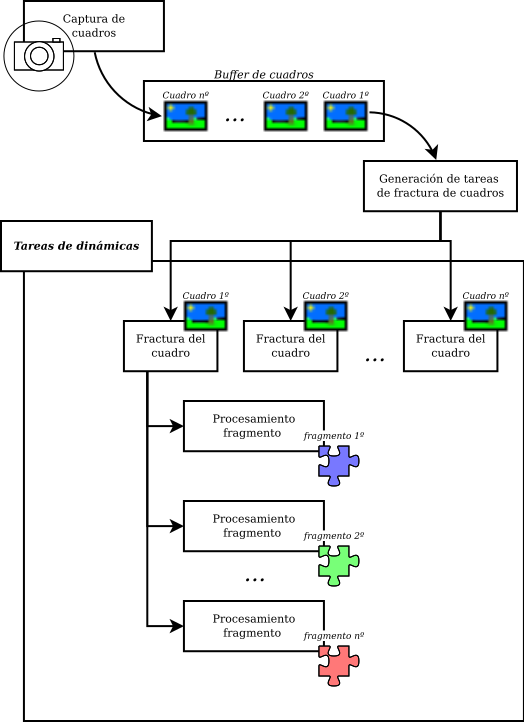
\includegraphics[width=\textwidth]{img/framework.pdf}

	\caption{Tareas principales del framework.}

	\label{tareasFramework}

\end{figure}

Cada una de las dos tareas estáticas tiene un hilo de ejecución asignado. Las
tareas dinámicas son ejecutadas por un conjunto de $N$ hilos de
ejecución\footnote{$N$ es un parámetro de entrada del programa.}. Cuando un hilo
de ejecución (del conjunto) está libre, toma una nueva tarea dinámica para
ejecutar. Como estos hilos de ejecución son los que ejecutan las tareas de
búsqueda, nos referiremos a ellos como "hilos de búsqueda". En la figura
\ref{tareasFramework} se muestran un diagrama de las tareas del framework, y en
la figura \ref{hilosFramework} se muestra como las tareas son asignadas a los
hilos de ejecución.

\begin{figure}[!h]

	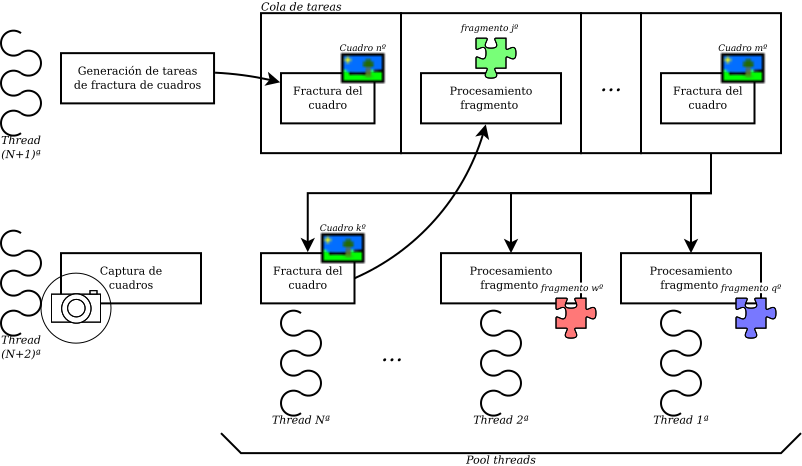
\includegraphics[width=\textwidth]{img/hilos.pdf}

	\caption{Asignación de tareas a los hilos de búsqueda.}

	\label{hilosFramework}

\end{figure}

Si el cuadro se divide en partes sin zonas solapadas puede suceder que los
parches de un robot se encuentren en fragmentos distintos. Esto es un problema,
ya que para encontrar los robots el plugin de detección de robots debe detectar
todos los parches que lo identifican, por lo cual todos deben estar dentro del
mismo fragmento. Para asegurar esto, cada par de fragmentos adyacentes deben
compartir una zona igual al diámetro de un robot. En la figura \ref{areaCompartida}
se muestran los casos donde el área compartida es menor al diámetro de un robot y
donde el área compartida es del diámetro de un robot.

\begin{figure}[!h]

	\centering
	
\includegraphics[width=0.45\textwidth]{img/areaTooSmall.pdf}
	
\includegraphics[width=0.45\textwidth]{img/areaPerfect.pdf}

	\caption{Izquierda: si el área compartida es demasiado pequeña y el
	robot se encuentra entre dos fragmentos, puede que sus parches no sean
	completamente visibles desde ninguno de ellos. Derecha: si el área
	compartida es del ancho de los robots, entonces todos los parches son
	visibles completamente desde por lo menos un fragmento.}

	\label{areaCompartida}

\end{figure}

Dado que los fragmentos comparten una área en sus bordes, la suma del área de
los fragmentos es superior al área de la imagen original. Para reducir los
píxeles a procesar, se debe reducir la zona compartida. Como la zona compartida
tiene un ancho fijo (el diámetro de un robot), para encontrar el área compartida
mínima se debe minimizar el perímetro del fragmento.

Por la manera que las imágenes se representan comúnmente en una computadora y
por su simplicidad, se opto por trabajar con un teselado con rectángulos. En el
caso de estos, para minimizar su perímetro y maximizar su área, se debe procurar
que la relación entre su ancho y altura sea lo mas cercana a uno. También,
para balancear la carga uniformemente, todos los fragmentos serán de igual
tamaño. Aquellos que se encuentren en los bordes inferior y derecho pueden que
sean mas chicos.

En la figura \ref{fragmentos} se muestran como se divide un cuadro de 800x600
píxeles con un área compartida de 50 píxeles en 1, 2, 5 y 8 fragmentos. Cuando
el número de fragmentos es un número primo, como en el caso de 5 fragmentos, el
cuadro se divide en franjas de igual ancho o altura que el cuadro original. Este
tipo de división produce fragmentos con perímetros mayores, produciendo grandes
áreas compartidas.

\begin{figure}[!h]

	
\includegraphics[width=0.5\textwidth]{img/fragmentos1.pdf}
	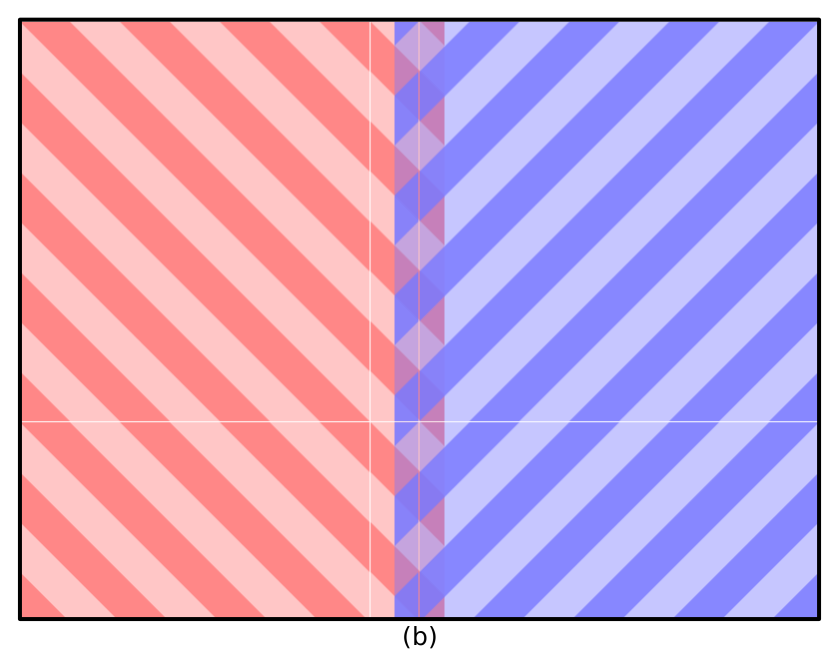
\includegraphics[width=0.5\textwidth]{img/fragmentos2.pdf}
	\includegraphics[width=0.5\textwidth]{img/fragmentos5.pdf}
	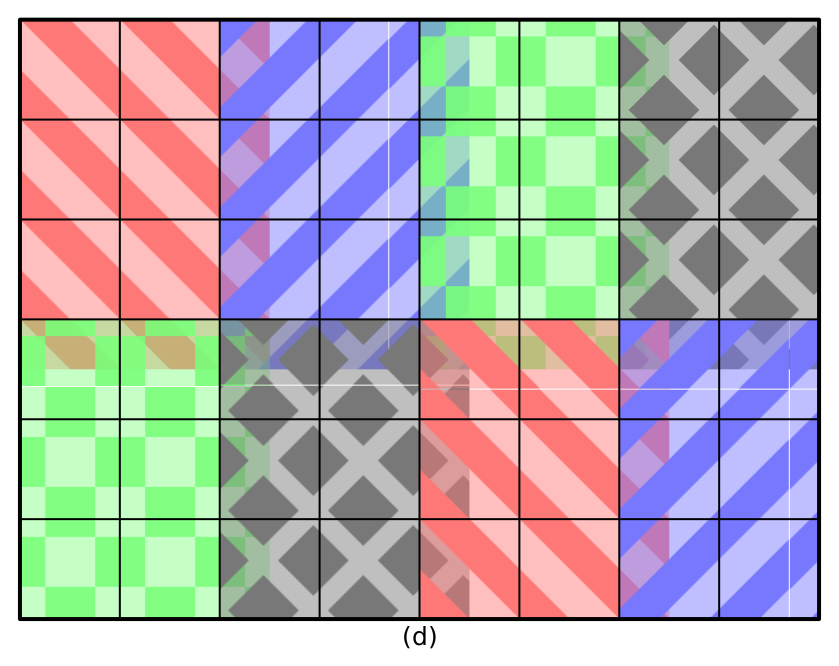
\includegraphics[width=0.5\textwidth]{img/fragmentos8.pdf}
	\caption{Resultado de dividir un cuadro de 800x600 píxeles con un área
	compartida de 50 píxeles en 1(a), 2(b), 5(c) y 8(d) fragmentos.}
	\label{fragmentos}

\end{figure}

\section{Implementación del framework}

El framework fue implementado en \emph{C++} con \emph{OpenMP} y está basada en
plugins para facilitar su modificación en un ambiente educativo.
La elección del lenguaje principalmente se debe a su eficiencia y paradigma.
Dado que el sistema debe procesar los cuadros en tiempos acotados, la eficiencia
es crucial, mientras que el paradigma orientado a objetos permite establecer
fácilmente la interfaz de los plugins. El uso de \emph{OpenMP} permite la
creación y control de hilos de ejecución y tareas de forma sencilla. Se
utilizaron los plugins implementados en \cite{torres2014}, modificándolos para
permitir su uso en un sistema paralelo.

\emph{OpenMP} es una API de bibliotecas y directivas al compilador para la
definición de paralelismo de alto nivel para sistemas de memoria compartida en
\emph{C}, \emph{C++} y \emph{Fortran}\cite{ompWeb}. La ventaja de \emph{OpenMP}
es que permite la creación de regiones paralelas, secciones criticas, tareas y
puntos de sincronización, simplemente marcando un bloque de código con unas
pocas directivas al compilador. \emph{OpenMP} ademas provee la facilidad de que
se puede establecer la cantidad de hilos que irán ejecutando las tareas, y que
el orden de la cola de espera es \emph{frist-come/first-served}. Aun así, en la
implementación final se mantiene un control del numero de tareas para no crear
mas de las que pueden ser procesadas, y no retrasar al sistema con tareas
viejas.

En la figura \ref{codigo} se muestra el fragmento de código (en pseudocódigo)
que ejecuta y crea las tareas principales del framework. La función principal
(\emph{main}, linea 1) del sistema comienza inicializando las estructuras del
sistema, incluyendo inicialización del sistema de captura y creación de plugins
y pilas de plugins entre otros. Se define también una estructura de control
compartida \emph{continuar} para indicar la finalización de la ejecución a las
tareas del sistema (linea 3). A continuación se crean tres hilos para la
ejecución de tres tareas (linea 4). La primer tarea es la generación de cuadros
(lineas 6 a 9), se llama al método de generación de cuadros dándole acceso a la
fuente de los cuadros (ya sea una cámara o un vídeo pre grabado), la pila de
cuadros y la estructura de control \emph{continuar}. La segunda tarea es la
tarea de generación de tareas de fragmentación de cuadros (lineas 10 a 14), se
llama al método de generación de tareas de fragmentación de cuadros, indicándole
la cantidad de hilos para tareas de búsqueda, la cantidad de partes en la que se
deben fragmentar los cuadros y dándole acceso a la pila de cuadros y la
estructura de control \emph{continuar}. La tercera tarea (lineas 15 a 18) se
encarga simplemente de esperar la señal de fin de ejecución (en el caso de los
experimentos espera a que pase un tiempo determinado), una ves que se cumple la
condición de corte, se pone en falso \emph{continuar}. En la finalización del
bloque de definición de tareas (linea 20) se define un punto de sincronización
tacito. Una ves que las tareas terminan, el sistema ejecuta el código de
finalización (linea 21).

La tarea de generación de tareas de fragmentación de cuadros se implementa en la
función \emph{generaciónDeTareasDeFragmentaciónDeCuadros} (lineas 25 a 71). La
función comienza estableciendo la cantidad de hilos de ejecución libres como la
cantidad de hilos de búsqueda (linea 28), luego se crean los hilos de búsqueda,
junto a uno más para la tarea de generación de tareas fragmentación de cuadros
(linea 29). La tarea de generación de tareas de fragmentación de cuadros consta
de un bucle que termina cuando la estructura de control \emph{continuar} es
falsa (lineas 31 a 68).

En cada iteración se verifica si hay hilos de ejecución libres y hay cuadros en
la cola de cuadros y de ser este el caso, se toma un cuadro de la pila de cuadros
(lineas 32 a 38). En caso de que se haya tomado un cuadro se reduce la cantidad
de hilos libres y se crea una tarea de fragmentación de cuadro con una copia
privada del puntero al cuadro (lineas 39 a 42).

La tarea de fragmentación de cuadro (lineas 43 a 66), comienza fraccionando el
cuadro y reservando un hilo por cada uno creado a partir del primero (lineas 45
a 47). Por cada cuadro se crea una tarea de procesamiento de fragmento (lineas
48 y 49).

Cada tarea de procesamiento de fragmento (lineas 50 a 58) procesa el fragmento
con cada pila (lineas 51 a 54). Antes de comenzar el procesamiento con cada pila
se reinician las estructuras del cuadro que sean necesarias (linea 52). Cuando
se termina de procesar el fragmento con todas las pilas se borra el fragmento
(linea 55) y se libera el hilo de ejecución (lineas 56 y 57).

La tarea de facturación de cuadro espera a la finalización de todas las tareas
de procesamiento de los fragmentos (linea 60), cuando terminan reserva un hilo
de ejecución (lineas 61 y 62), elimina el cuadro (linea 63) y libera el hilo de
ejecución (lineas 64 y 65).

\begin{figure}[!h]

	\includegraphics[height=\textheight]{img/itemSwitch.pdf}

	\caption{Pseudo código del sistema}

	\label{codigo}

\end{figure}

Las clases del framework básico son las siguientes:

\begin{description}

	\item[Item:] Esta clase define un tipo genérico de los ítems que serán
		tratados por el sistema.

	\item[RingBuffer:] Este es el buffer donde se guardan los ítems
		generados mientras esperan ser procesados. El buffer guarda solo
		punteros a objetos de la clase \emph{Item} y no tiene mecanismos
		de control que permitan acceder la estructura desde múltiples
		hilos al mismo tiempo de forma segura. Cuando se solicita un
		ítem, se devuelve el puntero al mas antiguo o \textbf{NULL} en
		caso de que la estructura este vacía. Cuando se intenta agregar
		un nuevo ítem pero la estructura esta llena, se coloca este en
		el espacio del ítem mas viejo en la estructura y se retorna el
		puntero de este al llamador, delegándole su destrucción. La
		destrucción del ítem se delega al llamador por dos motivos. El
		primero es que el buffer desconoce el tipo real del ítem. La
		segunda razón es que para poder ser utilizado de forma segura,
		las llamadas a los métodos del buffer deben estar dentro de
		secciones criticas y realizar las eliminaciones dentro de estas
		podría ser muy lento.

	\item[Input:] Se trata de una clase que funciona como definición de la
		interfaz de las clases que generan los ítems. Sus métodos
		principales son \emph{run} y \emph{generate}. El método
		\emph{generate} debe ser re implementado por las clases hijas
		para generar el tipo de ítem especifico del sistema. El método
		\emph{run} es el encargado de generar los ítems llamando a
		\emph{generate} y colocarlos en el \emph{RingBuffer}. Este
		último método puede ser redefinido si la aplicación así lo
		requiere.

	\item[ItemSlicer:] Es la clase que define la interfaz de las clases
		encargadas de dividir los ítems. Se definen tres métodos. El
		primero es \emph{slice} que recibe como parámetro ítem y la
		cantidad de partes en la que este debe ser dividido y retorna un
		arreglo de ítems. El segundo método es \emph{resetItem} que
		recibe como parámetro una de las partes creadas por el método
		\emph{slice} luego de que fue procesada por una pila de plugins
		y la configura al estado para que el funcionamiento de la
		próxima pila no se vea interferido. El tercer método es
		\emph{delPart} que recibe como parámetro un fragmento de ítem y
		lo elimina.

	\item[Plugin:] Esta clase define una interfaz para los plugins que
		realizaran las distintas partes del procesamiento de la imagen.
		Solo se define el método \emph{process} que tiene como único
		parámetro un puntero a un objeto de la clase \emph{Item}.

	\item[PluginStack:] Esta es la clase que tomara el ítem y se encarga de
		entregarlo a cada uno de los plugins. Tiene solo dos métodos,
		\emph{addPlugin}, para agregar un plugin, y \emph{process} que
		tiene como parámetro un ítem, para procesarlo.

	\item[ItemSwitch:] Esta es la clase encargada de implementar la tarea de
		generación de tareas de fragmentación de cuadro. Para no crear
		mas tareas de las que puede procesar el sistema, solo se toma un
		cuadro de la cola de cuadros a procesar si hay hilos de búsqueda
		libres y no hay tareas ya creadas para asignarles. Cada tarea de
		fragmentación de cuadro divide el ítem utilizando
		\emph{ItemSlicer} y crea una nueva tarea de procesamiento de
		cuadros por cada fragmento.

\end{description}

\begin{figure}[h]

	\includegraphics[width=\textwidth]{img/clasesFramework.pdf}

	\caption{Diagrama de clases Framework base.}

\end{figure}

Existen dos parámetros ajustables. El primero es la cantidad de hilos que
ejecutaran las tareas de búsqueda. El segundo parámetro es la cantidad de partes
en las cuales se dividirá el cuadro.

Para adaptar el framework para utilizarlo como un sistema de visión por
computadora para el fútbol de robots se incorporaron las siguientes clases, las
cuales fueron tomadas y modificadas del sistema de visión presentado en
\cite{torres2014}:

\begin{description}

	\item[Frame:] Subclase de \emph{Item}. Contiene una imagen que
		representa un cuadro y una estructura auxiliar que contiene la
		información necesaria para el funcionamiento de los plugins.

	\item[CaptureFromFile:] Subclase de \emph{Input}. Es la clase encargada
		de crear el flujo de objetos \emph{Frame}, tomando cada cuadro
		desde un archivo de vídeo. También debe respetar la taza de
		cuadros por segundo del vídeo.

	\item[FastCaptureFromFile:] Subclase de \emph{Input}. Muy similar a
		\emph{CaptureFromFile}, con las diferencias de que carga los
		cuadros a memoria antes de que comience el sistema a capturar
		los cuadros (para evitar los retardos de la lectura de disco y
		decodificación), y que tiene dos modos de controlar la
		frecuencia de la generación de los cuadros. Se puede adelantar
		la creación de cuadros si la cola de cuadros a procesar esta
		vacía, o fijar la frecuencia de su creación a un valor
		especifico. Esta clase es útil para comprobar la capacidad
		máxima del sistema, ya que permite simular una cámara con la
		velocidad de captura que se desee, y los distintos modos
		permiten testear la carga máxima en cuadros por segundo
		soportada por el sistema, así como los tiempos de espera bajo
		una cantidad de cuadros por segundo especifica.

	\item[FrameSlicer:] Subclase de \emph{ItemSlicer}. En este caso lo que
		se divide es la imagen del cuadro. Cada sub cuadro tendrá un
		solapamiento con los adyacente ya que se debe evitar que un
		robots o la pelota no este totalmente contenido dentro de por lo
		menos un sub cuadro. Para minimizar el área solapada, las
		particiones se realizan de manera tal que se minimice el
		perímetro pero ocupen la mayor área posible. Para lograr esto se
		busca la partición que haga que la relación entre el alto y el
		ancho sea lo mas cercana a uno.

	\item[Subclases de \emph{Plugin}:] \emph{PluginBlur},
		\emph{PluginColorConversions}, \emph{PluginColorSegmentation},
		\emph{PluginDetectBalls}, \emph{PluginFindBlobs},
		\emph{PluginFindSecondariesBlobs}, \emph{PluginMorphology} y
		\emph{PluginNetworking}.

	\item[Clases auxiliares:] \emph{ball}, \emph{colorspace},
		\emph{datastruct}, \emph{homography}, \emph{marker},
		\emph{pattern}, \emph{pattern\_matching},
		\emph{practicalsocket}, \emph{segmentation}, \emph{team},
		\emph{timer}.

\end{description}

\begin{figure}[h]

	\includegraphics[width=\textwidth]{img/clasesFrameworkRobots.pdf}

	\caption{Diagrama de clases del sistema sistema de visión para el fútbol
	de robots.}

\end{figure}

Conceptualmente, la implementación para fútbol de robots tiene dos pilas, una
para búsqueda de robots y la otra para búsqueda de la pelota. Sin embargo, ambas
pilas utilizan los mismos plugins con la misma configuración para la etapa de
pre procesamiento de la imagen, ademas, los plugins que no tienen en común solo
modifican datos propios de cada pila. Esto permite que ambas pilas puedan ser
unidas en una sola, lo que trae como ventaja que la etapa de pre procesamiento
se realice solo una ves por fragmento.
